
% 2 sadaļas, footeris, main content

Izstrādāto projektu ir iespējams uzstartēt ar \emph{shell} skriptu projekta
pamatdirektorijā -- \texttt{./start.sh}.
Projektu uzstartējot, apmeklējot ar interneta pārlūkprogrammu saiti
\url{https://127.0.0.1:5001/}, atvērsies lapa, kāda attēlota \ref{img:whole-ui} attēlā.

\begin{figure}[H]
	\centering
	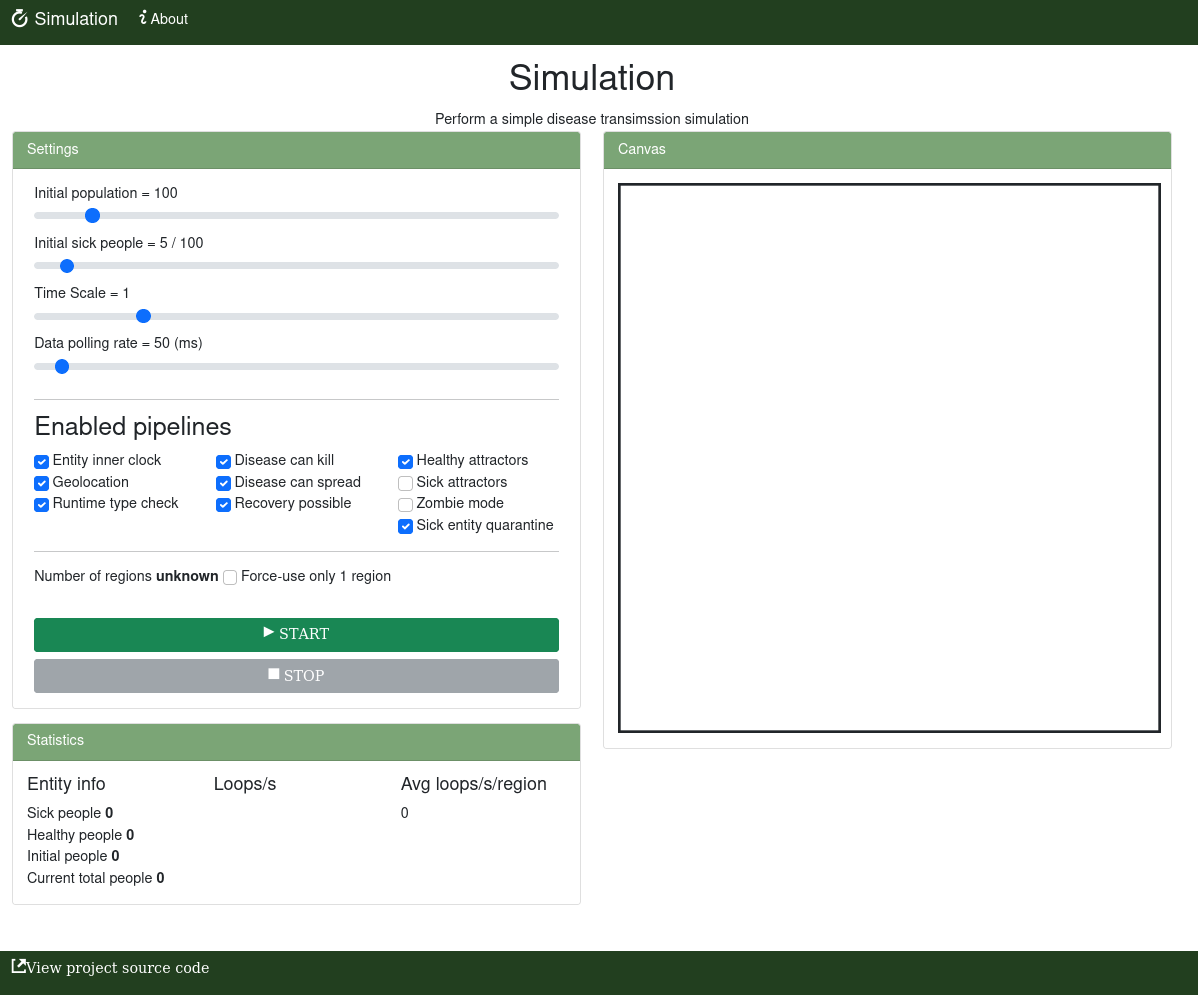
\includegraphics[scale=0.4]{images/ui-whole-page.png}
	\caption{Lietotāju saskarnes sākuma skats}
	\label{img:whole-ui}
\end{figure}

Lietotāju saskarne sastāv no divām lapām - pašas simulācijas (\ref{img:whole-ui}
att.) un ,,About" sadaļas (nav attēlots atskaitē).

% Settings panelis
\subsection{Iestatījumu panelis}

,,Settings" panelis (skat. \ref{img:settings} att.) ir galvenā vieta saskarnē,
kur ir iespējams veikt sekojošās darbības:

\begin{itemize}
    \item \emph{Pipeline} ieslēgšanu/izslēgšanu,
    \item populācijas skaita maiņu,
    \item slimo entītiju skaita maiņu,
    \item datu pieprasīšanas intervāla (\emph{polling rate}) maiņu,
    \item iespēja piespiedu kārtā izmantot tikai vienu \emph{Region} instanci
    \item uzsākt/apstādināt simulāciju.
\end{itemize}


\begin{figure}[H]
	\centering
	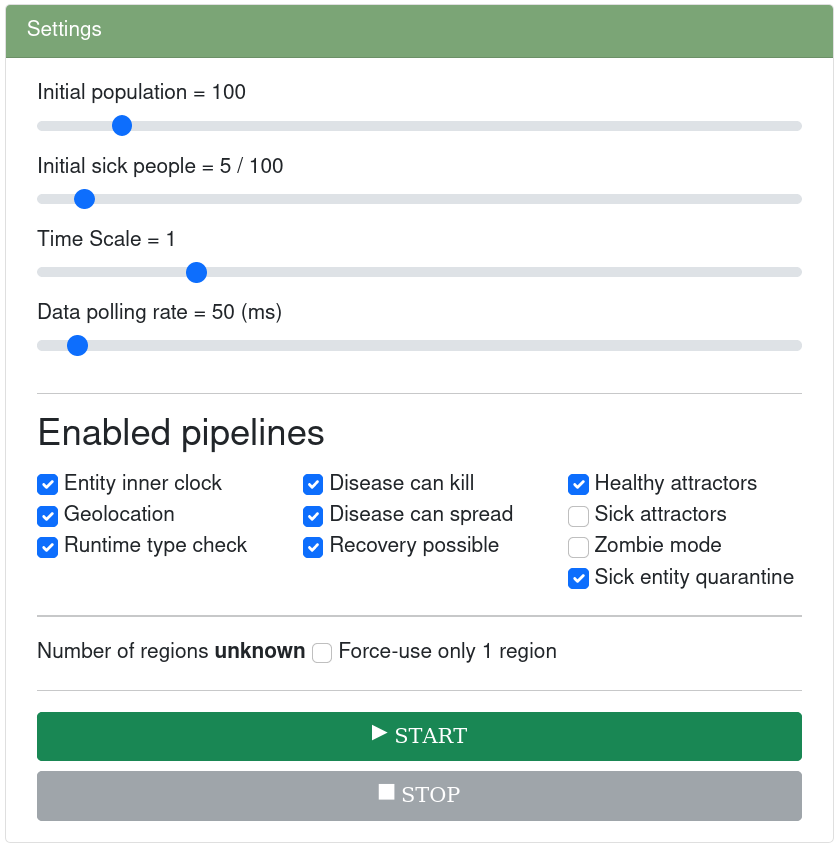
\includegraphics[scale=0.4]{images/settings.png}
	\caption{Iestatījumu panelis}
	\label{img:settings}
\end{figure}

% Canvas
\subsection{Kartes komponente}

\emph{Canvas} elements attēlo simulācijā esošos entītijus lietotājam. Ņemot vērā, ka
simulācijas plaknes izmēri nesakrīt ar pikseļu dimensijām lietotāju saskarnes
\emph{canvas} elementa izmēriem, tad katrs punkts arī tiek normalizēts jaunajās
(lietotājam redzamajās) dimensijās. Zināmas problēmas gan rodas gadījumos, kur
ir liels entītiju skaits -- \emph{JS Canvas 2d context API} nespēj pietiekami ātri
uzzīmēt lielo elementu skaitu, rodas vizuāli artefakti. \emph{Canvas} elementus
ar dažādiem simulācijas stāvokļiem dažādās stadijās var apskatīt \ref{img:canvas-show-off} attēlā.
Slimo entītiju krāsa mainās atkarībā no viņu veselības stāvokļa -- jo gaišāks, jo sliktāka veselība.

\begin{figure}[H]%
    \centering
    \subfloat
        [\centering Karantīna tiek ievērota (\emph{Healthy attractors} ieslēgts)]
        {{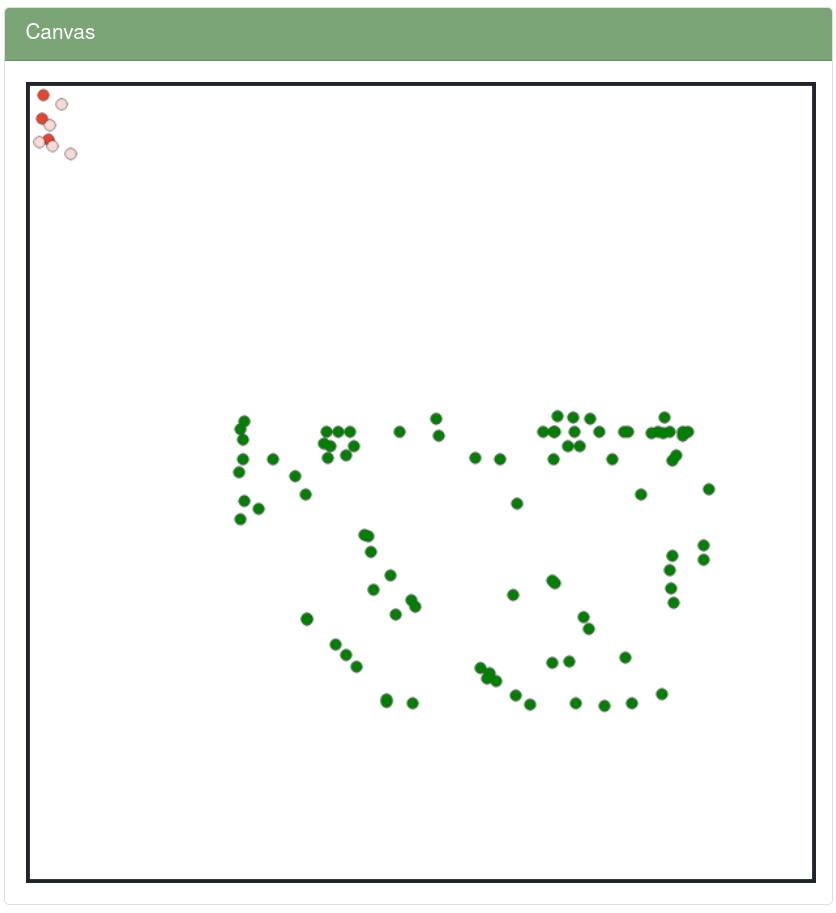
\includegraphics[width=.3\linewidth]{images/quarantine.png} }}%
    \qquad
    \subfloat
        [\centering Slimība izplatās, ja karantīna netiek ievērota]
        {{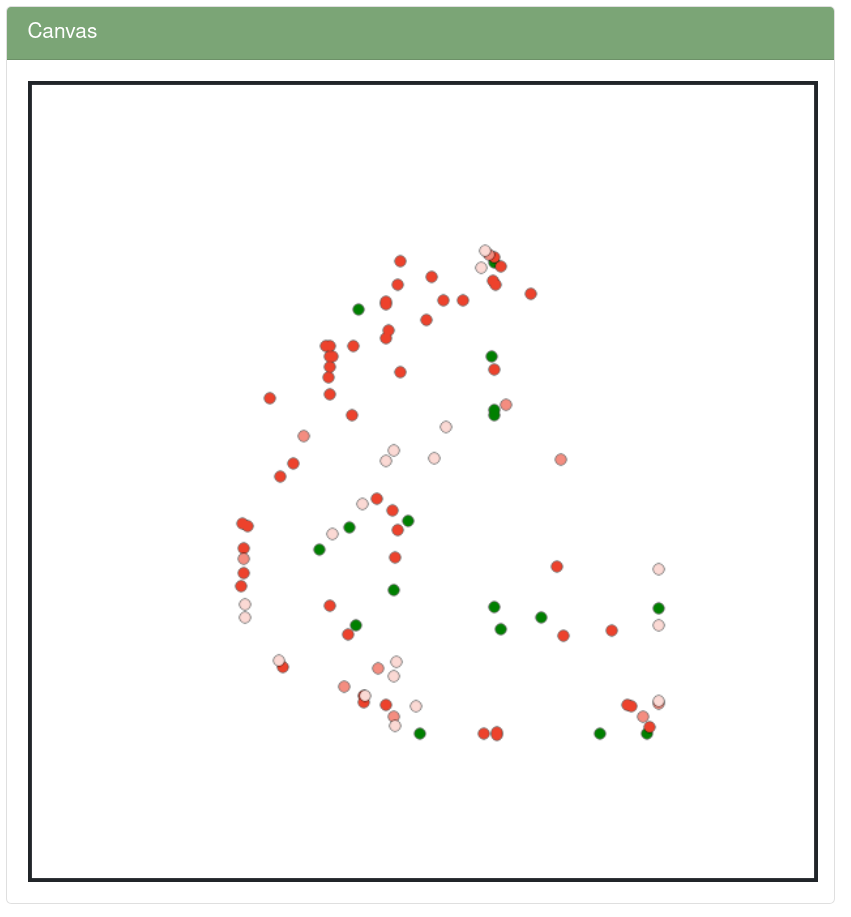
\includegraphics[width=.3\linewidth]{images/sickness-spreads.png} }}%
    \subfloat
        [\centering Atraktori ir izslēgti, ieslēgts \emph{Zombie mode}]
        {{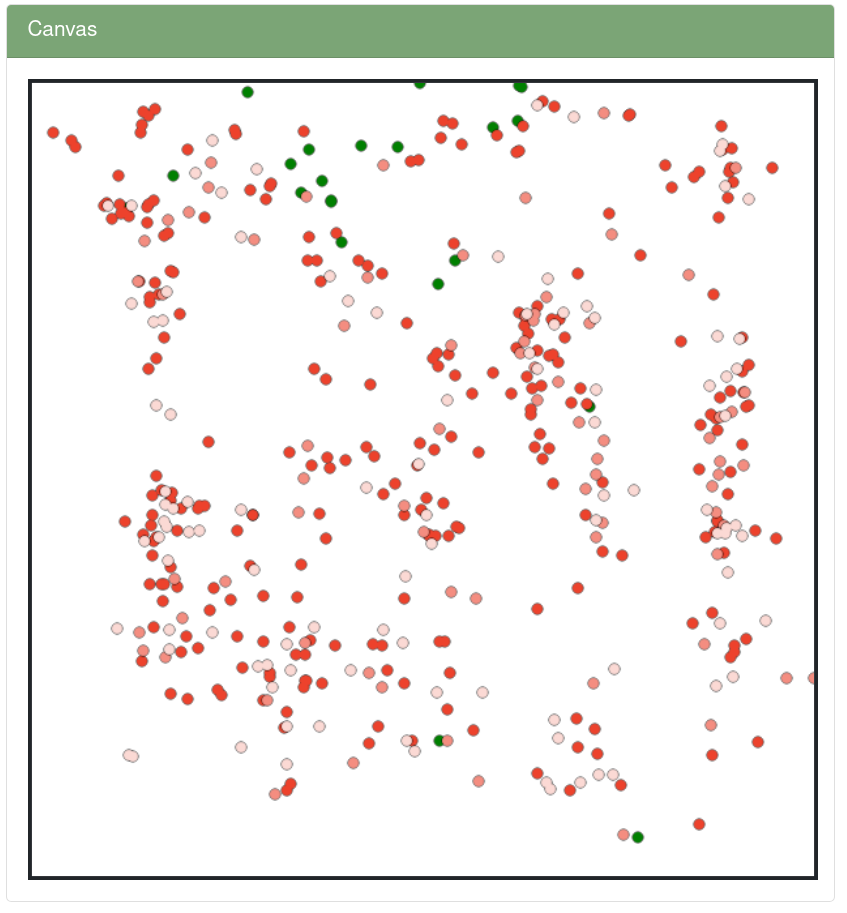
\includegraphics[width=.3\linewidth]{images/zombiemode-1.png} }}%
    \qquad
    \subfloat
    [\centering Ilgtermiņā turot ieslēgtu \emph{Zombie mode}, var redzet \emph{Region} sadalījumu]
        {{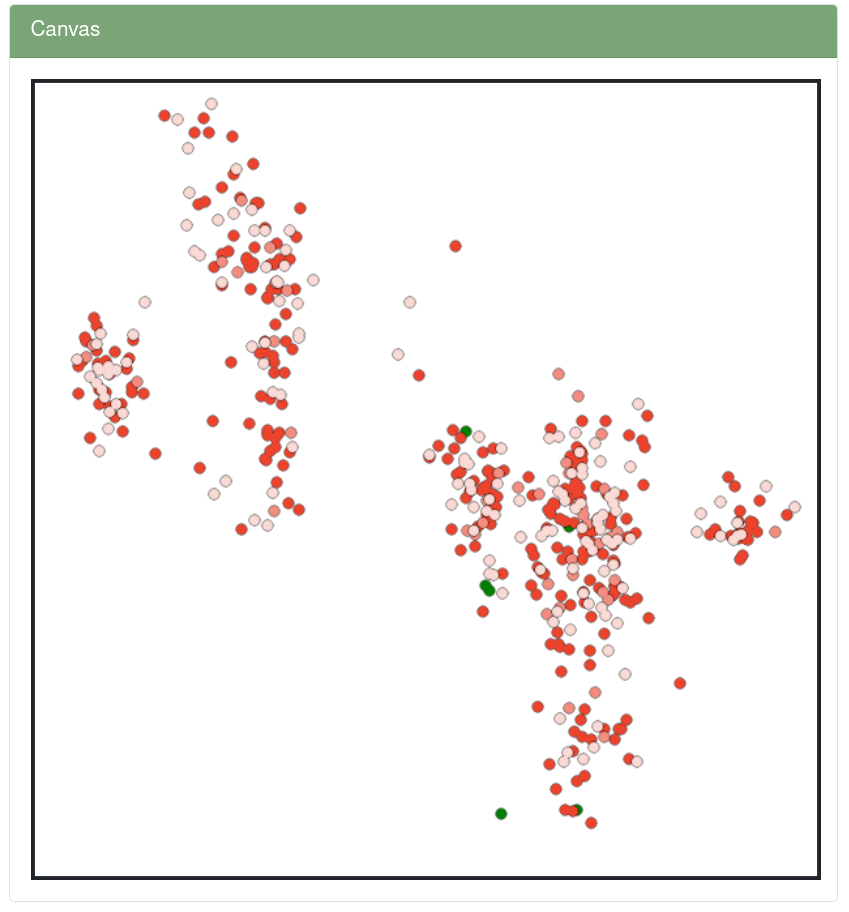
\includegraphics[width=.5\linewidth]{images/zombiemode-2.png} }}%
    \caption{Dažādu simulācijas stāvokļu vizualizācija}%
    \label{img:canvas-show-off}%
\end{figure}

% Statistics
\subsection{Statistikas komponente}

Tā kā \emph{canvas} vizualizācija der tikai kā uzskates materiāls, tad \emph{Statistics}
sadaļa atļauj apskatīt to, kas notiek sistēmā skaitliskā veidā (skat. \ref{img:statistics} att.).
Šī sadaļa ir sadalīta 3 kolonnās -- entītiju vispārīgā statistika, katra reģiona
noslodze, kas tiek mērīta ar iterācijām sekundē, kur 1 iterācija ir:

\begin{itemize}
    \item visu reģiona entītiju izlaišana caur \emph{pipeline},
    \item \emph{inbound} bufera pārbaude,
    \item entītiju ievietošana \emph{out of bounds} buferī.
\end{itemize}

3. kolonna šajā komponentē ir vidējais aritmētiskais visu reģionu
noslodzei kopš simulācijas sākuma. Šie skaitļi atļauj ērti analizēt sistēmas
izmaiņas pie dažādiem iestatījumiem.

\begin{figure}[H]
	\centering
	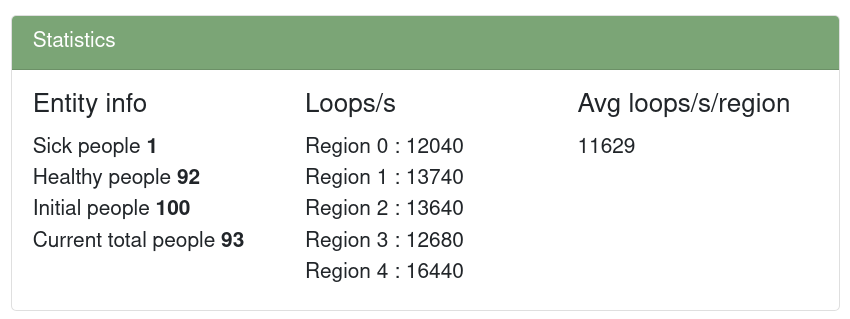
\includegraphics[scale=0.5]{images/statistics.png}
	\caption{Statistikas sadaļa}
	\label{img:statistics}
\end{figure}

% Max entities, no deaths, no nothing 1REGION vs 5 REGIONS
\subsection{Vairāku-kodolu stresa tests}

Izmantojot šo informāciju, kas apskatāma \emph{Statistics} komponentē, var veikt
nelielus testus esošajai programmai. Sākotnējais entītiju skaits tika uzlikts uz
maksimālo, lai pēc iespējas vairāk noslogotu procesoru, tad tika palaista programma
apmēram 20 sekundēm, tikai ievākta informācija no sistēmas. Šāda procedūra tika
atkārtota, izmantojot 1 \emph{Region} un 5 \emph{Region} instances. Rezultātus
ir iespējams apskatīt \ref{img:test-single-vs-mutlicore} attēlā.

\begin{figure}[H]%
    \centering
    \subfloat
        [\centering Statistika ar 1 \emph{Region} instanci]
        {{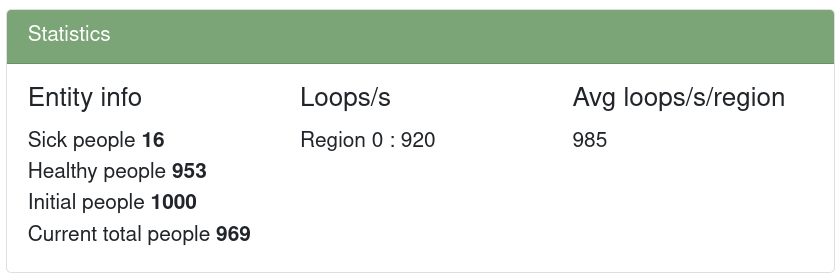
\includegraphics[width=.7\linewidth]{images/stress-statistics-single-sm.png} }}%
    \qquad
    \subfloat
        [\centering Statistika ar 5 \emph{Region} instancēm]
        {{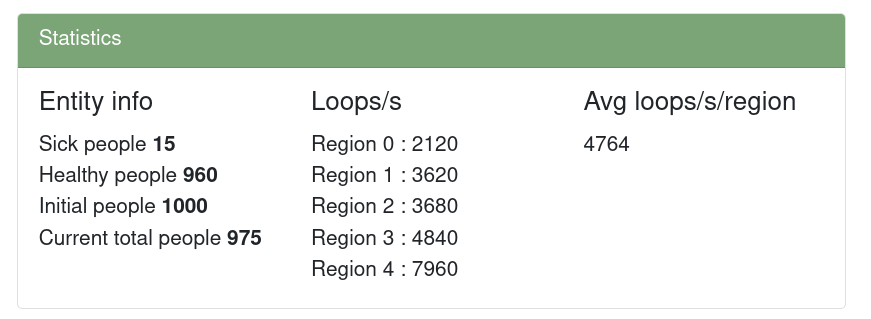
\includegraphics[width=.7\linewidth]{images/stress-stastiscs-multiple.png} }}%
    \caption{Sistēmas stresa tests}
    \label{img:test-single-vs-mutlicore}%
\end{figure}

Informāciju, ko attēlo šī komponente ir jāvērtē tikai kā ,,ieskats". Katru
reizi ģenerējot jaunu simulāciju, entītijas tiek uzģenerētas citās vietās, ar
dažādiem parametriem, sistēmas \emph{atraktori} tiek definēti dažādos daudzumos
un dažādās vietās.
Protams, to visu ir iespējams statiski iekodēt kodā, lai tas nemainās, tad veiktu
testus, tomēr,
izstrādājot sistēmu, mērķis nebija veikt padziļinātu analīzi par paralelizācijas
uzlabojumiem.
